\begin{minipage}[t]{180mm}
\fcolorbox{black}{white}{
\begin{minipage}[b]{30mm}

\includegraphics[width=0.5\linewidth]{unflogo.pdf}
\end{minipage}
\begin{minipage}[b]{100mm}
\Huge \textbf{UNF NEWZ} \\
\Large -- Søvn og retsstavning er overvurderet! 
\end{minipage}
\begin{minipage}[b]{50mm}
\Large Onsdag 17.07.2015 \\
\normalsize Redigeret i \LaTeX\ af \\ SOM, MGS, MMN, SABH
\end{minipage}
}
\end{minipage}



\begin{minipage}[b]{0.95\linewidth}
\begin{minipage}[t]{0.47\textwidth}
\vspace{3mm}
\section*{Dagens fysiker}
Hvis du møder en fysiker, så prik ham, og fortæl, at du har tjekket, at hans kat er død.

\section*{Ordforklaring: Kat}
Internettet (hvis vi ser bort fra nulmængder)

\begin{center}
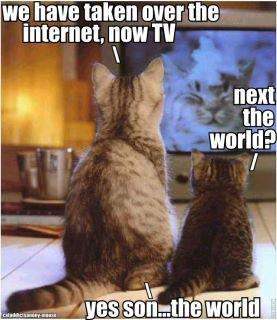
\includegraphics[width=0.6\textwidth]{Cats.jpg}
\end{center}

\end{minipage}%
\hfill\begin{minipage}[t]{0.47\textwidth}
\vspace{3mm}
\section*{Vejrudsigt}
\textbf{IMF, AU (fra DMI)}: Få skyer og en del sol. Op til 21 grader om dagen og ned til 11 grader om natten, ingen regn og vind fra vest.

\textbf{S 56 W 170}: Koldfront med støt sydvind og høje bølger.

\section*{Find en Fynbo}
På trods af en klapjagt i nattens mørke er Fynboen endnu ikke fundet, og der frygtes, at han igen gemmer sig i denne avis. Der er udlagt brunsvigerfælder, men øjensynligt har Fynboen medbragt egne rationer.

\section*{Fakta om Jylland}
Når en jyde siger, at noget er ringe, er det ikke nødvendigvis også grupper.

\section*{Dagens sandsynlighed}
Sandsynligheden for at gå fallit, ved at spille roulette ubegrænset længe med begrænsede penge, er $1$.

\vspace{3mm}
\end{minipage}

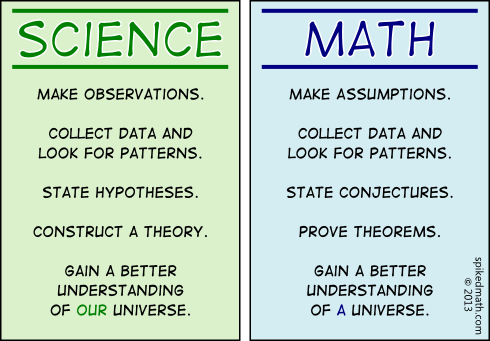
\includegraphics[width=\textwidth]{542-science-vs-math.png}
\begin{center}
\tiny Mike, http://spikedmath.com/542.html, CC-BY-NC-2.5

\vspace{3mm}

\tiny UNF Newz er avisen, hvor ansvarshavende redaktør fralægger sig ethvert ansvar for eventuel plagiat, kaniner, tysk, stavefelj, kaffe, dårlig humor, glemsomhed, katte, store sigmaer, pile, skyer, dårlige oversættelser og alt, hvad eventuelle Homo sapiens sapiens kunne finde på at holde imod UNF Newz! Dog tager UNF Newz fuld credit og copyright for alle guldkorn, magickort, mus, \TeX, humor, smil, Mortener, kaffe, før-fremtid, ringe og/eller rubik's cube.
\end{center}
\end{minipage}

